\chapter{Simulations of galaxy clusters}\label{clustersim}
\section{Details of the simulations}
We performed two simulations of cluster formation with Enzo following
\citet{Iapichino2008}. One simulation was done with the Schmidt SGS model
including the Sarkar corrections and some additional modifications described
below. For comparsion we conducted a second simulation without SGS model. In the
following section we describe the common features of these two simulations, in
section \ref{numissues} we describe some additional numerical issues, which had
to be taken into account when doing a cluster simulation with SGS model in
comoving coordinates. 
\subsection{Common features}\label{common}
The simulations were done using a flat (critical density $\Omega=1$) cold dark
matter (CDM) background cosmology with a dark energy density
$\Omega_{\Lambda}=0.7$, a total (including baryonic and dark matter) matter
density $\Omega_{m}=0.3$, a baryonic matter density $\Omega_{b}=0.04$, the
Hubble parameter set to $h=0.7$, a galaxy fluctuation amplitude $\sigma_8=0.9$,
and a scalar spectral index $n=1$. Both simulations were started with the same
initial conditions at redshift $z_{ini}=60$, using the \citet{Eisenstein1999}
transfer function, and evolved to $z=0$. The simulations were adiabatic with a
heat capacity ratio $\gamma=5/3$ assuming a fully ionized gas with a mean
molecular weight $m_{\mu}= \unit[0.6]{u}$. Cooling physics, magnetic fields,
feedback, and transport processes are neglected. 

The simulation box had a comoving size of $\unit[128]{Mpc\ h^{-1}}$. It was
resolved with a root grid (level $l=0$) of $128^3$ cells and $128^3$ N-body
particles. A static child grid ($l=1$) was nested inside the root grid with a
size of 
64 Mpc/h, $128^3$ cells and $128^3$ N-body particles. The mass of each particle
in this grid was $\unit[9 \times 10^9]{M_{\odot}\ h^{-1}}$. Inside this grid, in
a volume of $\unit[38.4]{Mpc\ h^{-1}}$, adaptive grid refinement from level
$l=2$ to $l=6$ was enabled using a overdensity refinement criteria as described
in \citet{Iapichino2008} with an overdensity factor $f=4.0$. The refinement
factor between two levels was set to $r=2$, allowing for a effective resolution
of $8196^3$ cells or $\unit[15.6]{kpc\ h^{-1}}$.

The static and dynamically refined grids were nested around the place of
formation of a galaxy cluster, identified by \citet{Iapichino2008} using the
HOP algorithm \citep{Eisenstein1998}. The cluster had a virial mass of
$M_{vir}=\unit[5.49 \times 10^{14}]{M_{\odot}\ h^{-1}}$ and a virial radius of
$R_{vir}=\unit[1.33]{Mpc\ h^{-1}}$ for both simulations.  

\subsection{Numerical issues}\label{numissues}
Running robust simulations including a SGS model like the Schmidt or Sarkar
model in a comoving cosmological background requires some additional techniques
not yet discussed. Apart from the additional terms due 
to comoving coordinates in the filtered equations, these techniques help to
handle the extreme high turbulent Mach numbers, which appear on the coarsest
grids in these simulations and are briefly described in the following sections.

\subsubsection{Filtered equations of fluid dynamics in comoving coordinates}
Filtering the equations of fluid dynamics in comoving coordinates
\eqref{eq:commass2}-\eqref{eq:cometot2} can be done in the same way as
filtering the equations in cartesian coordinates as shown in chapter \ref{FE}.
As a result we get
\begin{align}
\pd{t}\fil{\tilde{\rho}} + \fa\pd{x_j}\hat{u}_j \fil{\tilde{\rho}} =& 0,
\label{eq:filcommass2}\\
\begin{split}
\pd{t}\fil{\tilde{\rho}} \hat{u}_i 
+ \fa\pd{x_j}\hat{u}_j \fil{\tilde{\rho}} \hat{u}_i =& 
-\fa\pd{x_i}\fil{\tilde{p}}+ \fa\pd{x_j}\fil{\sigma'_{ij}} 
+\fil{\tilde{\rho}}\hat{g}^*_i 
-\fa\pd{x_j}\hat{\tau}(u_i,u_j)\\
&- \fh \fil{\tilde{\rho}} \hat{u}_i,
\label{eq:filcommom2}
\end{split}
\\
\begin{split}
\pd{t}\fil{\tilde{\rho}}e_{res}+\fa\pd{x_j}\hat{u}_j\fil{\tilde{\rho}}e_{res}=&
-\fa\pd{x_i}\hat{u}_i\fil{\tilde{p}}
+\fa\pd{x_j}\hat{u}_i\fil{\sigma'_{ij}}
+\fa\fil{\tilde{\rho}}\hat{u}_i\hat{g}^*_i\\
&-\fh(\fil{\tilde{\rho}}e_{res}
+\frac{1}{3}\fil{\tilde{\rho}}\hat{u}_i\hat{u}_i+\fil {\tilde{p}})\\
&+\fil{\tilde{\rho}}(\lambda+\epsilon)
-\fa\hat{u}_i\pd{x_j}\hat{\tau}(u_i,u_j)
-\fa\pd{x_j}\hat{\tau}(u_j,e_{int}),\label{eq:filcomresetot}
\end{split}
\\
\pd{t}\fil{\tilde{\rho}}e_t+\fa\pd{x_j}\hat{u}_j\fil{\tilde{\rho}}e_t=&
\mathbb{D} +\Gamma
-\fil{\tilde{\rho}}(\lambda+\epsilon)
-\fa\hat{\tau}(u_j,u_i)\pd{x_j}\hat{u_i}
-2\fh\fil {\tilde{\rho}}e_t.
\label{eq:filcomet}
\end{align}

In the source code of Enzo the derivatives are always taken with respect
to $r_i=a x_i$ and the additional terms due to comoving coordinates in 
momentum and resolved energy equation are already implemented. So the only term
we had to implement additionally compared to the non-comoving case was the term
$2\fh\fil {\tilde{\rho}}e_t$ in the equation of turbulent energy. Furthermore
for the subgrid model terms it is necessary to take into account that
the Jacobian of the velocity in comoving coordinates is\footnote{See equation
\eqref{eq:cotrans5} in the Appendix.}
\begin{align}
J_{ij} = \pd{r_i}v_j&=\fa\pd{x_i}u_j + \fh\delta_{ij}.
\end{align}
The tracefree rate of strain tensor in comoving coordinates for example can then
be easily expressed in terms of the Jacobian of the velocity field
\begin{align}
S^*_{ij}=\frac{1}{2}\lra{J_{ij}+J_{ji}}-\frac{1}{3}\delta_{ij}J_{kk}.
\end{align}
Basically all terms in the subgrid model using derivatives of the resolved
velocity are therefore written in terms of the Jacobian of the velocity.

\subsubsection{Turbulent energy cutoff and lower limit for temperature}
High turbulent Mach numbers occur in cosmological simulations especially in the
very cold, low-density voids of the computational domain. To make sure that in
our adiabatic simulation the temperature and therefore the sound speed doesn't
drop to unphysical low values we introduced a lower limit of the temperature
$T_{min}=\unit[10]{K}$. This value is reasonable, since no gas in the
universe can have a temperature lower than the cosmic microwave background
temperature of 2.7 K for a longer time. Since there are presumably more
heating mechanisms like UV-heating, choosing 10 K as a lower limit seems to be
a rational choice. 

On the other side, low density gas can be accelerated very quickly in a
gravitating field, leading to high velocity gradients, which lead to 
production of high amounts of turbulent energy according to the turbulent
viscosity hypothesis. However the validity of the turbulent viscosity
hypothesis has never been tested or verified in astrophysical
flows. We are therefore free to assume that for flows with high velocity
gradients, the production of turbulent energy is restricted and use as an
upper limit of the turbulent Mach number $M_{t,max}=\sqrt{2}$. The exact value
of this limit is based on the idea that in an isothermal gas (speed of sound 
$c_{\text{s,iso}} = \frac{p_{th}}{\rho}$), the total pressure can be expressed as
\begin{align}
p_{tot}=\rho c_{\text{s,iso}}^2 + \frac{1}{3}\rho q^2 = \gamma_{\text{eff}} \rho c_{\text{s,iso}}^2.
\end{align}
If we assume that $\gamma_{\text{eff}}$ is not allowed to be higher than the
adiabatic value $\gamma=5/3$, we have to limit the isothermal turbulent Mach number to
$\frac{q}{c_{\text{s,iso}}} \leq \sqrt{2}$.  

\subsubsection{Treatment of shocks}
Shocks form unavoidably during cosmological structure formation due to
infalling plasma which accretes onto filaments, sheets, and halos, as well as
due to supersonic flows associated with merging substructures
\citep{Pfrommer2006}. But shocks are the most localized and anisotropic
features of a flow and therefore cannot be treated by an SGS model, which 
is based on the assumption of isotropy of the flow on the subgrid
scales.\footnote{Also see chapter \ref{amrles}.} So in principle, shocks should
be treated by the mechanisms of AMR alone and the SGS model should
not influence the shocks. That's why we implemented a simple shock detector
\begin{align}
-\ppd{r_i}{v_i} l_{\Delta} > c_s,
\end{align}
which marks all cells, where the velocity increments are greater than the
speed of sound, as shocks. At these cells, we disable the SGS model, which
means no production or dissipation of turbulence takes place. The turbulent
energy is only advected in these cells.   

\section{Results}
\subsection{Energy conservation}
Energy conservation is crucial for any adiabatic fluid dynamic simulation.
However it is difficult to test for this directly in our setup, since we cannot
extract easily the energy injected by gravity into the system. By plotting the
time development of the mass weighted mean total energy in the system, which is
for the simulation without SGS model the sum of mass weighted mean internal
energy and mass weighted mean kinetic energy and for the simulation with Sarkar
model the sum of mass weighted means of internal, kinetic and turbulent energy,
we can still gain some insights into the differences between the two
simulations. 

\begin{figure}[tp]
\centering
\includegraphics[width=0.7\linewidth]{chapter9/energyerror.eps}
\caption{Time development of total energy in cluster simulation with and
without SGS model.}
\label{fig:etot}
\end{figure}

This is what has been done in figure \ref{fig:etot}. From it we can see
that the time development of the total energy is nearly identical, if we take
the turbulent energy into account when computing the total energy of the
simulation with Sarkar model. On the other side, the difference between the sum
of kinetic and internal energy between the simulations seems to be again mostly
accounted for by the turbulent energy, a result similar to what was already
found in the simulations of driven turbulence.\footnote{See section
\ref{numenergy}.}
We can also infer from figure \ref{fig:etot}, that the SGS model mainly changes
the ratio of mean internal to mean kinetic energy and does not have much
influence on the mean potential energy of the system. However, this is to be
expected, since most of the gravitational potential is due to dark matter
anyway, and we do not model the influence of gravity on subgrid scales and vice
versa in our SGS model. This leads us to conclude that the general effects of
our SGS model in a selfgravitating fluid are very similar to the effects found
in the driven turbulence simulations without self gravity.  

\subsection{Mass fractions of different gas phases}
The IGM on large scales of the universe can be classified roughly into four
phases according to gas temperature: the hot gas with $T > \unit[10^7]{K}$
inside and around clusters; the warm-hot intergalactic medium (WHIM) with
$\unit[10^5]{K} < T < \unit[10^7]{K}$ found mostly in filaments; the low
temperature WHIM with $\unit[10^4]{K} < T < \unit[10^5]{K}$ distributed mostly
as sheetlike structures; and the diffuse cold gas with $T < \unit[10^4]{K}$
residing mostly in voids \citep{Cen1999,Kang2005}. To investigate the influence
of the SGS model on these different gas phases, we plotted the time development
of the mass fractions according to each of the phase for the simulation with
and without SGS model (figure \ref{fig:massfrac1a} and \ref{fig:massfrac1b}).
\begin{figure}[tp]
\centering
\subfigure[No SGS model.]{
\includegraphics[width=0.45\linewidth]{chapter9/mass_red_nosgs.eps}
\label{fig:massfrac1a}}
\subfigure[SGS model.]{
\includegraphics[width=0.45\linewidth]{chapter9/mass_red_sar.eps}
\label{fig:massfrac1b}}
\caption{Time development of mass fractions of different gas phases in the
whole simulation box had with a comoving size of
$\unit[128]{Mpc\ h^{-1}}$.}
\end{figure}
We also show the mass fractions of each gas phase at redshift $z=0$ in table
\ref{tab:massfrac1}. 
\begin{table}[htbp]
\begin{center}
\begin{tabular}{lcccc}
\hline
Run & 
$\frac{m_{\text{cluster}}}{m_{\text{all}}}\ [\%]$ &
$\frac{m_{\text{filaments}}}{m_{\text{all}}}\ [\%]$ &
$\frac{m_{\text{sheets}}}{m_{\text{all}}}\ [\%]$ & 
$\frac{m_{\text{voids}}}{m_{all}}\ [\%]$ \vspace*{1mm} \\
\hline
\hline
no SGS & 5.50 & 40.3 & 4.22 & 49.1\\ 
SGS & 5.47 & 37.5 & 3.28 & 53.0 \\
\hline
\end{tabular}
\end{center}
\caption{Mass fractions of different gas phases at redshift $z=0$.}
\label{tab:massfrac1}
\end{table}
The results seem to indicate that the SGS model leads to higher mass fraction
of the voids and a lower mass fraction of the filaments compared to the
simulation without SGS model. However our simulation domain is not very well
resolved outside the central region, since we do not allow for adaptive
refinement there. If we restrict our analysis to the adaptively refined region
in the box with a size of $\unit[38.4]{Mpc\ h^{-1}}$, the differences between
the simulation with SGS model and without SGS model vanish 
(figure \ref{fig:massfrac2a} and \ref{fig:massfrac2b}).
\begin{figure}[tp]
\centering
\subfigure[No SGS model.]{
\includegraphics[width=0.45\linewidth]{chapter9/mass_red_nosgs_small.eps}
\label{fig:massfrac2a}}
\subfigure[SGS model.]{
\includegraphics[width=0.45\linewidth]{chapter9/mass_red_sar_small.eps}
\label{fig:massfrac2b}}
\caption{Time development of mass fractions of different gas phases in the
centered subset of the simulation box with a comoving size of 
$\unit[38.4]{Mpc\ h^{-1}}$. One can see that the total mass in this open region
is not conserved.}
\end{figure}
This can also be seen from the mass fractions at redshift $z=0$ normalized to
the total mass in the central region in table \ref{tab:massfrac2}. 
\begin{table}[htbp]
\begin{center}
\begin{tabular}{lcccc}
\hline
Run & 
$\frac{m_{\text{cluster}}}{m_{\text{all}}}\ [\%]$ &
$\frac{m_{\text{filaments}}}{m_{\text{all}}}\ [\%]$ &
$\frac{m_{\text{sheets}}}{m_{\text{all}}}\ [\%]$ & 
$\frac{m_{\text{voids}}}{m_{all}}\ [\%]$ \vspace*{1mm} \\
\hline
\hline
no SGS & 19.2 & 40.8 & 2.61 & 37.5\\ 
SGS & 19.0 & 40.1 & 2.64 & 38.2 \\
\hline
\end{tabular}
\end{center}
\caption{Mass fractions of different gas phases at redshift $z=0$ for the
adaptively refined region with a size of $\unit[38.4]{Mpc\ h^{-1}}$.}
\label{tab:massfrac2}
\end{table}
From these results we conclude that the SGS model has no or only very little
influence on the mass fractions of the different gas phases in the simulations.
For the important mass fraction of the WHIM we get $ \approx 38\%$, which is 
higher than found by \citet[simulation B1]{Dave2001} ($ \approx 32\%$) with a
lower resolution AMR simulation, but lower than found by \citet{Gottlober2006}
($ \approx 40\%$), who used smoothed particle hydrodynamic (SPH) with 
$2 \times 1024^3$ particles to simulate a box of size $\unit[500]{Mpc\ h^{-1}}$;
so we are also consistent with the literature in this respect.

\subsection{Development of turbulence in different gas phases}
The eddy turnover time $t_l$ associated with a scale $l$ 
\begin{align}
t(l) = \frac{l}{q(l)}
\end{align}
is the typical time for a structure of size $\sim l$ to undergo a significant
distortion due to turbulent motions characterized by the
typical turbulent velocity $q(l)$ at that scale \citep{Frisch1995}. So if we
divide the age of the universe $t(z)$ by the eddy turnover time, we get the
number of eddy turnovers 
\begin{align}
n(l,z)=\frac{t(z)}{t(l)}
\end{align}
at a given redshift $z$ at a scale $l$. If $n > 1$, there has been enough time 
for eddies of size $l$ to cascade down to smaller scales and we can call the
fluid turbulent at scale $l$. 

In static grid simulations one often chooses to use the grid resolution
$l_{\Delta}$ as characteristic length scale and to compute a characteristic
velocity and eddy turnover time for this scale. However in an AMR code it is not
trivial to compute the turbulent velocity $q_l$ associated with a characteristic
length scale $l = l_{\Delta}$, since $l_{\Delta}$ is varying in time and space.
To circumvent this difficulty, we assume that below the grid resolution at a
certain position turbulent velocity scales according to Kolmogorov
\begin{align}
q(l) \sim l^{1/3}.
\end{align}
We thereby assume that locally, the cascade starts at a different length scale
characterized by the different resolution of our grid at that position. We also
assume that our refinement criterion tracks and finds the regions inside the
fluid, which do not scale according to Kolmogorov, and refines them until a
Kolmogorov scaling is reached. Of course one might doubt that our refinement
criterion based on overdensity will accomplish that. But since in cosmological
simulations gravity is basically the energy-injecting force in the fluid and
gravity is strongest in regions of high density, one can argue that in regions
of high density, the Kolmogorov cascade starts at smaller length scales and
the energy injecting scales in these regions have to be refined with a finer
grid. Of course a criterion solely based on density might be necessary,
but is not at all sufficient to track regions of Non-Kolmogorov scaling.
More research needs to be done in this direction, but it is outside of the 
scope of this work. 

For the analysis in our work, we adopt the hypothesis of local Kolmogorov
scaling below the grid resolution. As a characteristic scale of our analysis,
we choose the length scale of our highest resolved regions, which is 
$l_{min}=\unit[15.6]{kpc\ h^{-1}}$. The turbulent velocity in the highest
resolved regions can be directly computed from the values of the turbulent
energy $q(l) = \sqrt {2 e_t}$ on the grid; the turbulent velocity in less
refined regions is scaled down according to our local Kolmogorov hypothesis as
\begin{align}
q(l_{min}) = q(l_{\Delta}) \lra{\frac{l_{min}}{l_ {\Delta}}}^{1/3}
\label{eq:vturbscaled}.
\end{align}
Using this scaled turbulent velocity to compute the eddy turnover time, we 
plotted the mean mass weighted number of eddy turnovers at $l_{min}$ with
respect to redshift (see figure \ref{fig:eddy}). 
\begin{figure}[tp]
\centering
\includegraphics[width=0.7\linewidth]{chapter9/eddy_red_sar.eps}
\caption{Mean number of eddy turnovers for gas phases of
different temperature over time.}
\label{fig:eddy}
\end{figure}
We can clearly see from this graph, that starting from a redshift $z=2$ all gas
phases are turbulent at the scale $l_{min}=\unit[15.6]{kpc\ h^{-1}}$. We also
see that the amount of turbulence in terms of eddy turnover times is higher in
regions of higher temperature and therefore highest in the cluster gas.    

Another important measure for turbulence is the turbulent Mach number
introduced in section \ref{dimanalsgs}. Like the eddy turnover time, the
turbulent Mach number is scale dependent
\begin{align}
M_t(l)=\frac{q(l)}{c_s}.
\end{align}
In figure \ref{fig:machturb} we plot the mean mass weighted turbulent Mach
number characteristic for the scale of our analysis 
$l_{min}=\unit[15.6]{kpc\ h^{-1}}$ making again use of our local Kolmogorov
hypothesis.
\begin{figure}[tp]
\centering
\includegraphics[width=0.7\linewidth]{chapter9/machturb_red_sar.eps}
\caption{Mean turbulent Mach number at a scale 
$l_{min}=\unit[15.6]{kpc\ h^{-1}}$ for gas phases of different temperature over
time.}
\label{fig:machturb}
\end{figure}
It is evident that the turbulence at $l_{min}$ is subsonic in all gas phases
during the whole time of the simulation. At redshift $z=0$ the average
turbulent Mach number is $\approx 0.2$. If the
amount of turbulence would be equal in each gas phase one would expect the
turbulent Mach number to scale $\sim 1/c_s \sim 1/\sqrt{T}$. However this is
not the case. The cluster gas is much more turbulent than estimated by this
simple scaling relation; in fact there is more turbulent energy compared to 
internal energy in the hottest gas phase than in the WHIM, although there is a
substantial drop of the turbulent Mach number between redshift $z=1-2$. The
drop in turbulent Mach number is presumably due to heating of the cluster gas
during a phase of major mergers at that time. In the next section, we will 
present some further evidence for this interpretation.  

\subsection{Scaling of turbulent energy}
In chapter \ref{numtest} we studied the scaling of the turbulent energy
with the resolution and were able to show that the scaling
of turbulent energy in our simulations of driven turbulence actually follows
the Kolmogorov scaling law. In this section we repeat this analysis for our 
cluster simulation. Figure \ref{fig:tuerescluster} shows the time development of
the mass weighted mean turbulent energy for every level of our AMR simulation. 
\begin{figure}[tp]
\centering
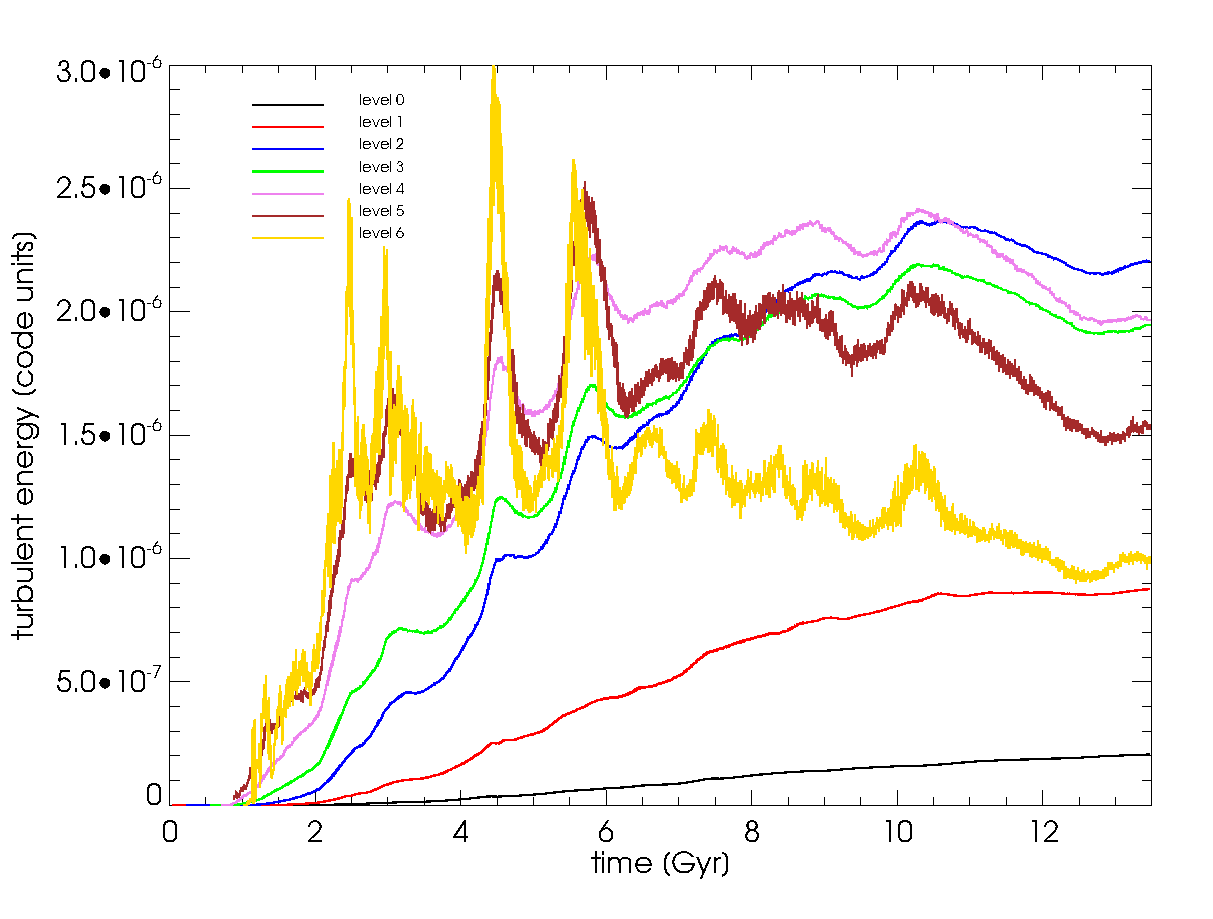
\includegraphics[width=0.7\linewidth]{chapter9/tuemwrescluster128sar.eps}
\caption{Time development of mean turbulent energy over time for each level of
refinement.}
\label{fig:tuerescluster}
\end{figure}
We see from the plot, that the turbulent energy on the higher levels (meaning
at smaller scales) is higher at times $t<\unit[6]{Gyr}$. Later this picture
changes, but not completely. For example the turbulent energy on level 4 stays
above the turbulent energy of level 3 for the whole simulation time. Also
striking are the high fluctuations in the time $\unit[2]{Gyr}<t<\unit[6]{Gyr}$,
which correspond to a redshift $z=3-1$ of the turbulent energy at the smaller
scales. This is also the time when the turbulent Mach number inside the
cluster drops significantly (see last section), so we can interpret these high
fluctuations as further evidence for violent major mergers, that happen at that
time, producing turbulent energy, which is then dissipated into internal energy
heating up the cluster gas. However at the time $t>\unit[13]{Gyr}$, the
simulation seems to reach some kind of stable state, similar to what is found in
driven turbulence simulations. We therefore can compute mean turbulent energies
by averaging the turbulent energy from $t=\unit[13]{Gyr}$ to the end of the
simulation and plot them against the grid length scale of the associated level.
The result (in terms of the turbulent velocity) can be seen in figure 
\ref{fig:tuefitcluster}. 
\begin{figure}[tp]
\centering
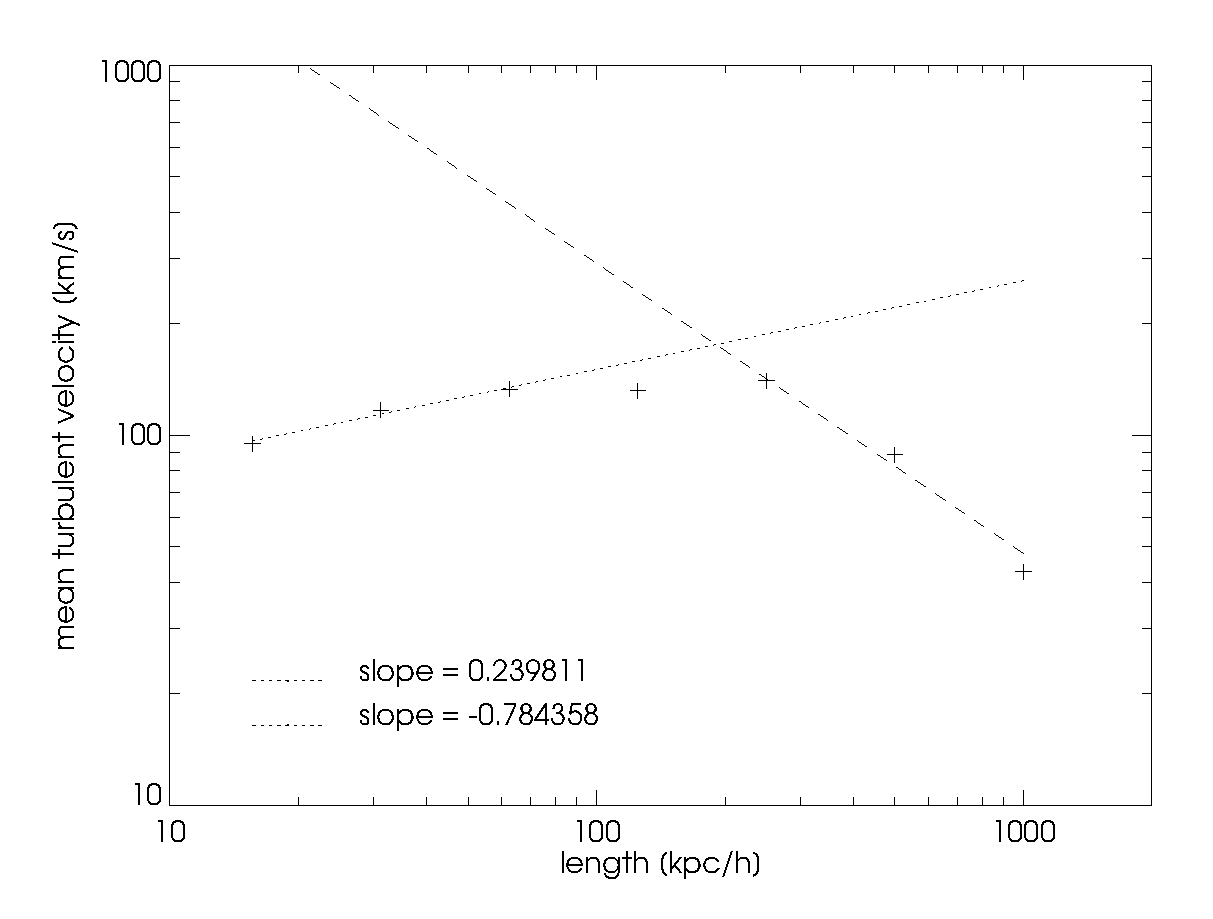
\includegraphics[width=0.7\linewidth]{chapter9/tuemwfitcluster128.eps}
\caption{Scaling of mean turbulent energy. The dotted line is a fit showing the
scaling behavior of turbulent energy below $\unit[100]{kpc\ h^{-1}}$, the dashed
line is a fit showing the scaling behavior above $\unit[100]{kpc\ h^{-1}}$.}
\label{fig:tuefitcluster}
\end{figure}
It is obvious that this is no Kolmogorov scaling. However, we do not expect to
see a Kolmogorov scaling again, since, as explained in the last section, we
assume the resolved regions to be non-Kolmogorov anyway. Still the result is
interesting, showing a peak in the turbulence around $\unit[100]{kpc\ h^{-1}}$
and a drop off towards higher and smaller scales. Also shown in the figure are
power-law fits, which gave a scaling of $q \sim l^{-0.78}$ for scales bigger
than $\unit[100]{kpc\ h^{-1}}$ and a scaling of $q \sim l^{0.24} \sim l^{1/4}$
for smaller scales. If one wants to interpret this result in terms of a
turbulent cascade, one could say that up to a length scale of  
$\unit[100]{kpc\ h^{-1}}$, energy is injected into the system, cascading down
towards smaller scales with a scaling behavior $q \sim l^{1/4}$ flatter than
expected for a Kolmogorov scaling with $q \sim l^{1/3}$. But, assuming our local
Kolmogorov hypothesis holds, it would follow, that below the grid resolution
of $\unit[15.7]{kpc\ h^{-1}}$ the cascade should be Kolmogorov again. Of course
a interpretation like this is highly speculative; much more data on
turbulence in cluster simulations is necessary to show that the
observed power-law scalings are real indeed.

\subsection{Radial profiles of the cluster}
As mentioned in section \ref{common}, the simulation is centered around a
galaxy cluster with a virial mass of $M_{vir}=\unit[5.49 \times
10^{14}]{M_{\odot}\ h^{-1}}$ and a virial radius of $R_{vir}=\unit[1.33]{Mpc\
h^{-1}}$ for both simulations, which center is identified using the
HOP algorithm. In the following we present plots of radial profiles of several
quantities around the center of this cluster (figure
\ref{fig:dens}-\ref{fig:vturb})
obtained by using a modified version\footnote{We modified \texttt{enzo\_anyl} to
allow plotting of SGS model quantities like the turbulent velocity.} of the
\texttt{enzo\_anyl} tool, which is part of the public Enzo release.   
\begin{figure}[tp]
\centering
\subfigure[Gas density.]{
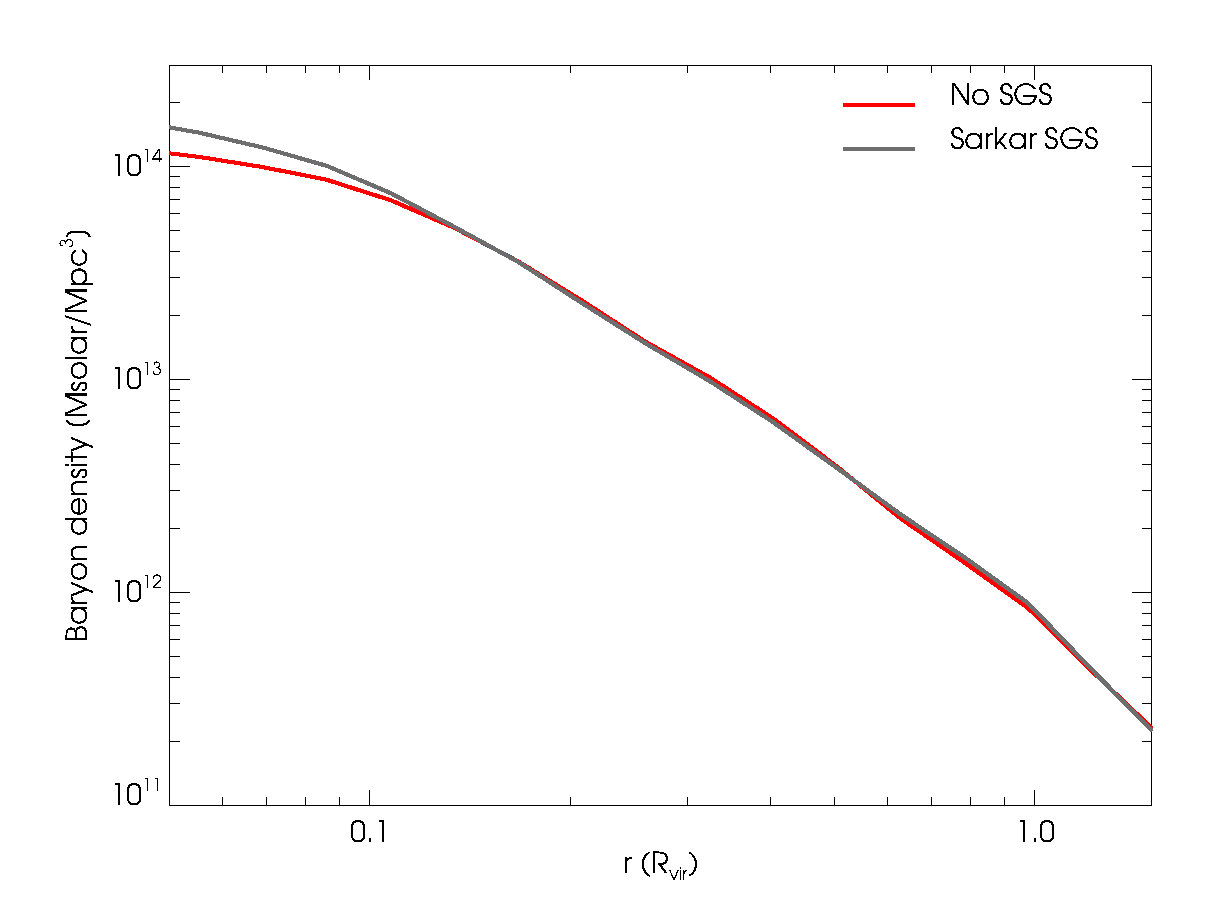
\includegraphics[width=0.45\linewidth]{chapter9/d_gaslog.eps}
\label{fig:dens}}
\subfigure[Temperature.]{
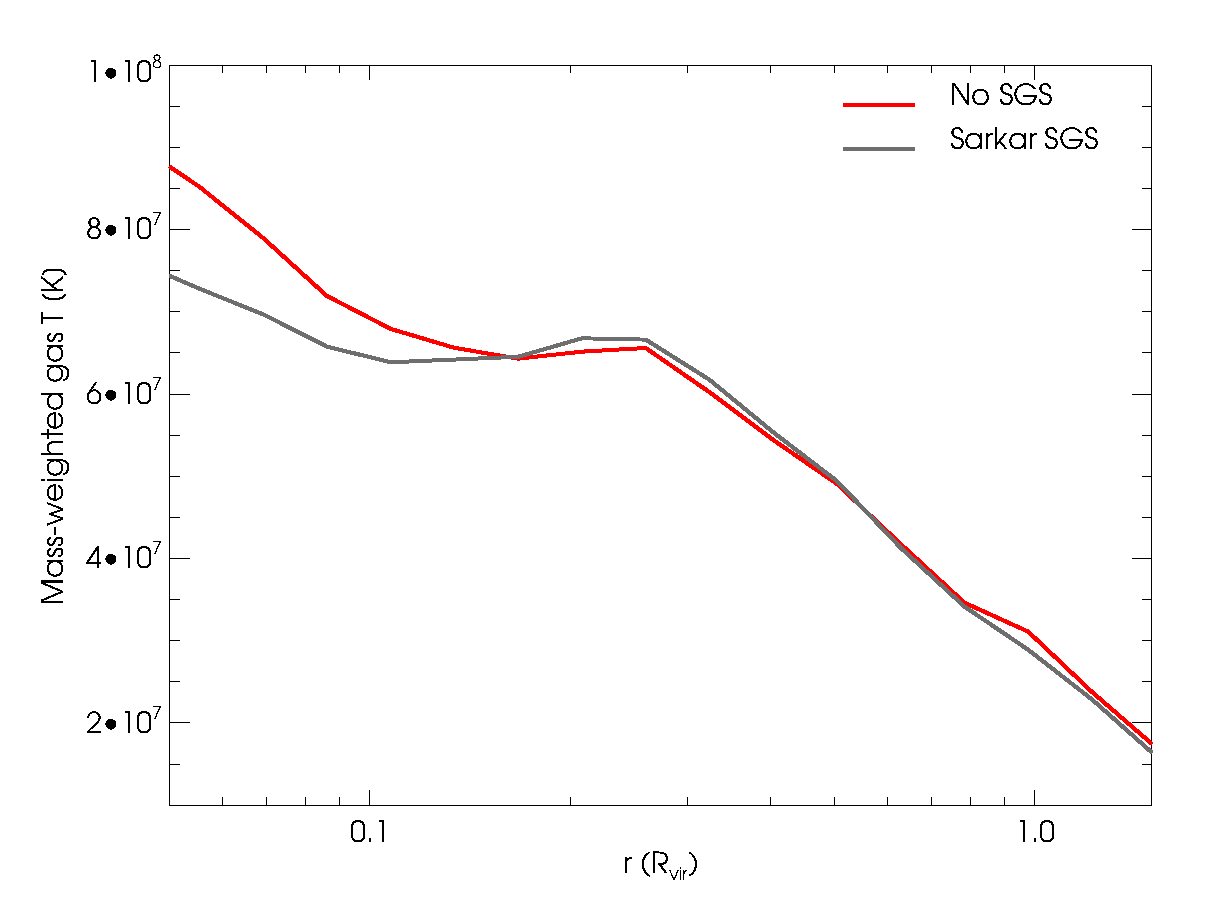
\includegraphics[width=0.45\linewidth]{chapter9/templog.eps}
\label{fig:temp}}
\subfigure[Entropy.]{
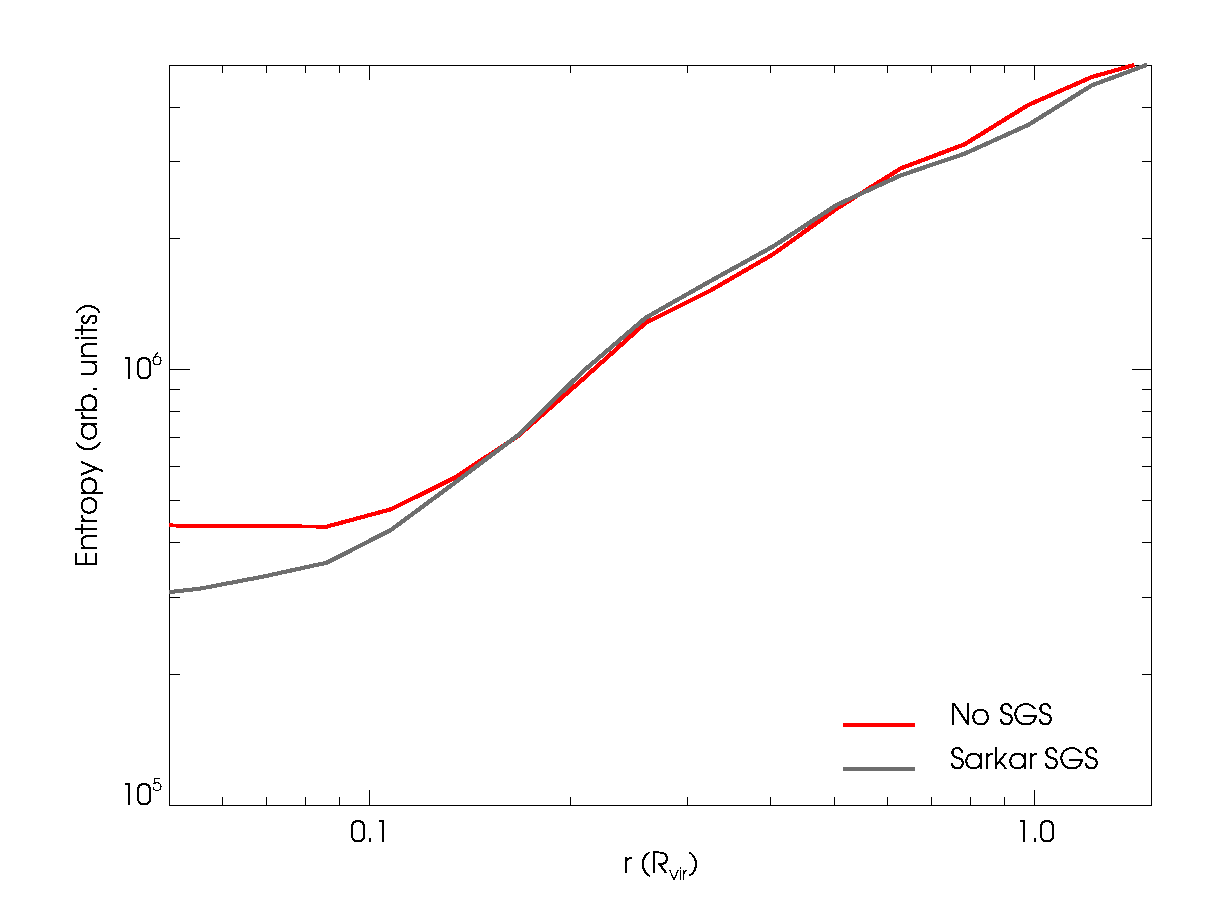
\includegraphics[width=0.45\linewidth]{chapter9/entropylog.eps}
\label{fig:entro}}
\subfigure[X-ray luminosity.]{
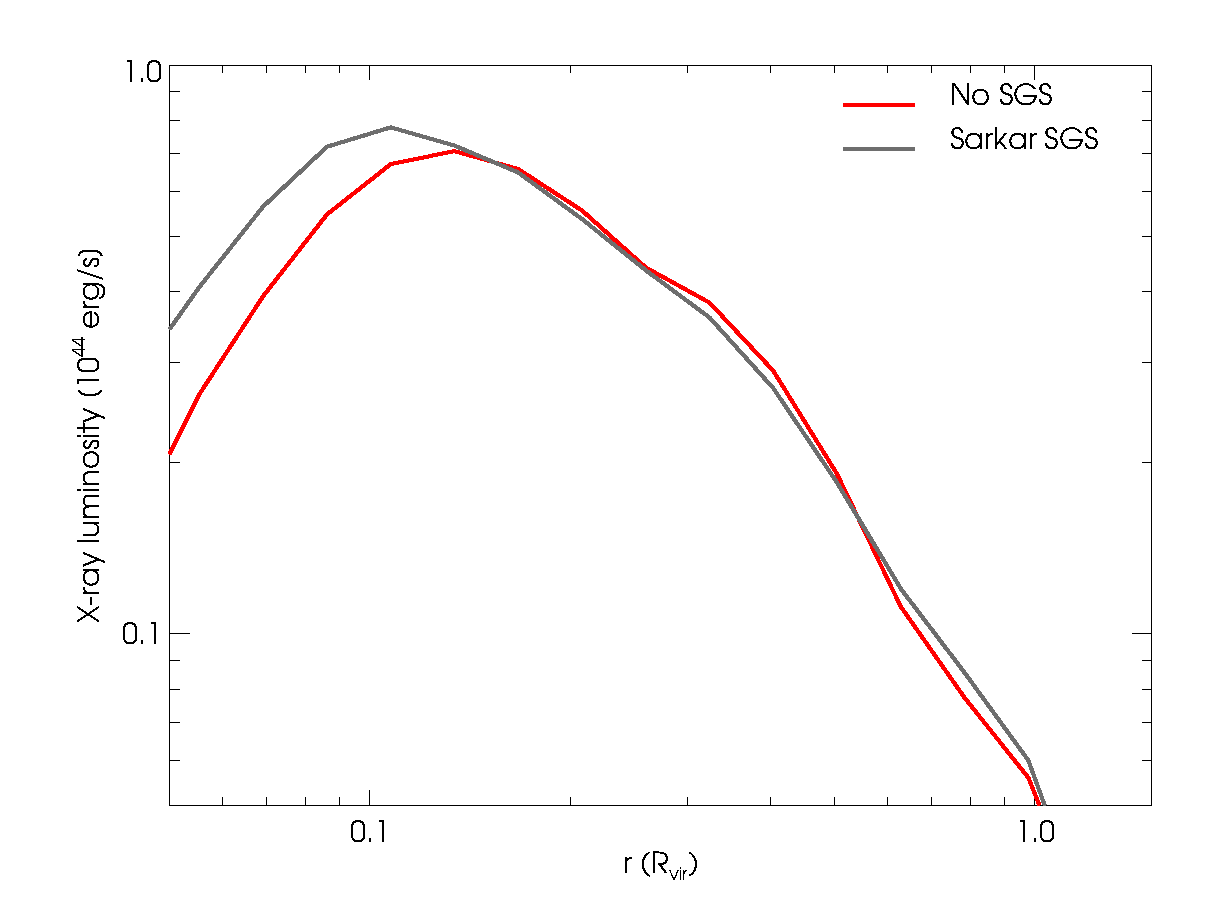
\includegraphics[width=0.45\linewidth]{chapter9/xraylog.eps}
\label{fig:xray}}
\subfigure[Radial profile of effective polytropic index $n_{\text{eff}}(r)$.]{
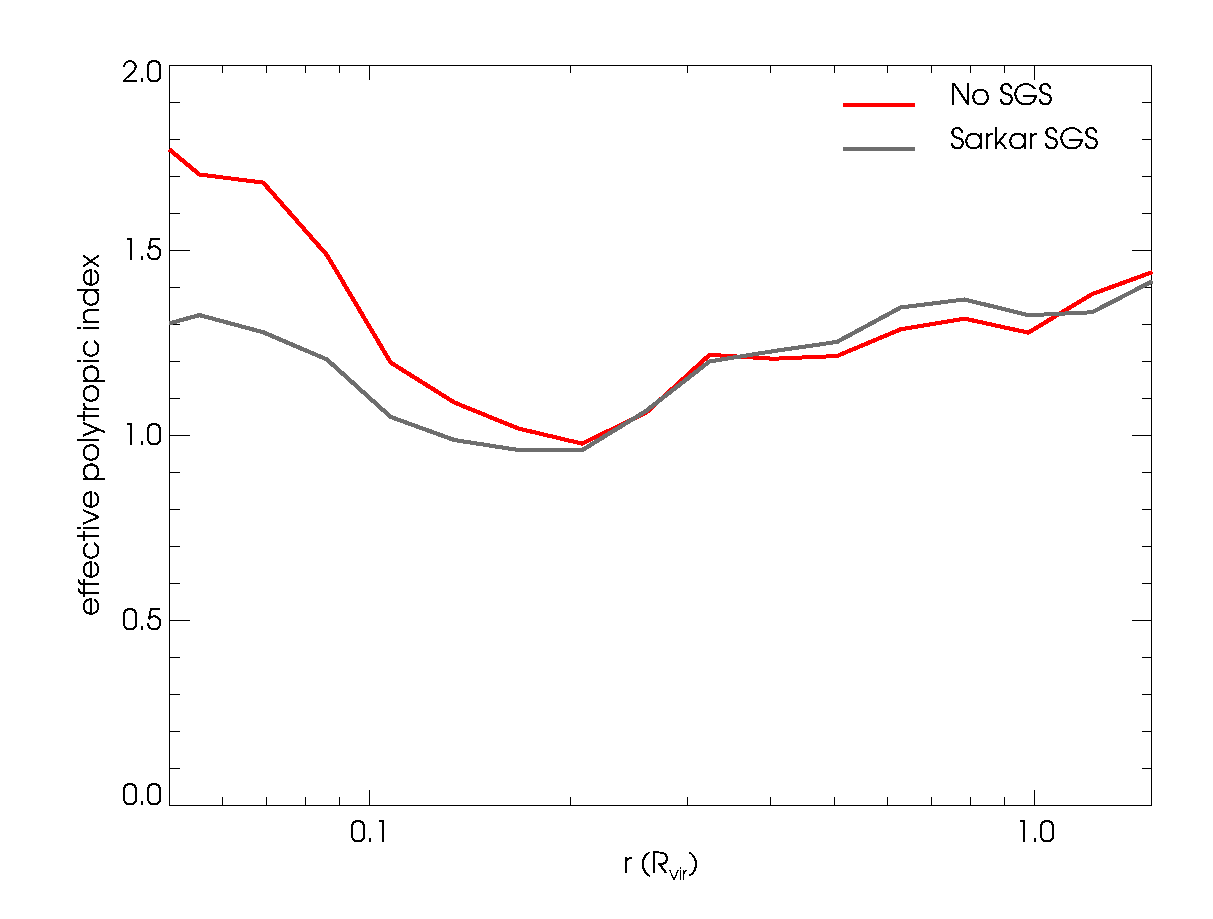
\includegraphics[width=0.7\linewidth]{chapter9/gamma.eps}
\label{fig:poly}}
\caption{Radial profiles of several thermodynamic quantities around the center
of the galaxy cluster. The results for the simulation with and without Sarkar
SGS model are
plotted in red and black respectively.}
\end{figure}
\begin{figure}[tp]
\centering
\subfigure[Radial velocity.]{
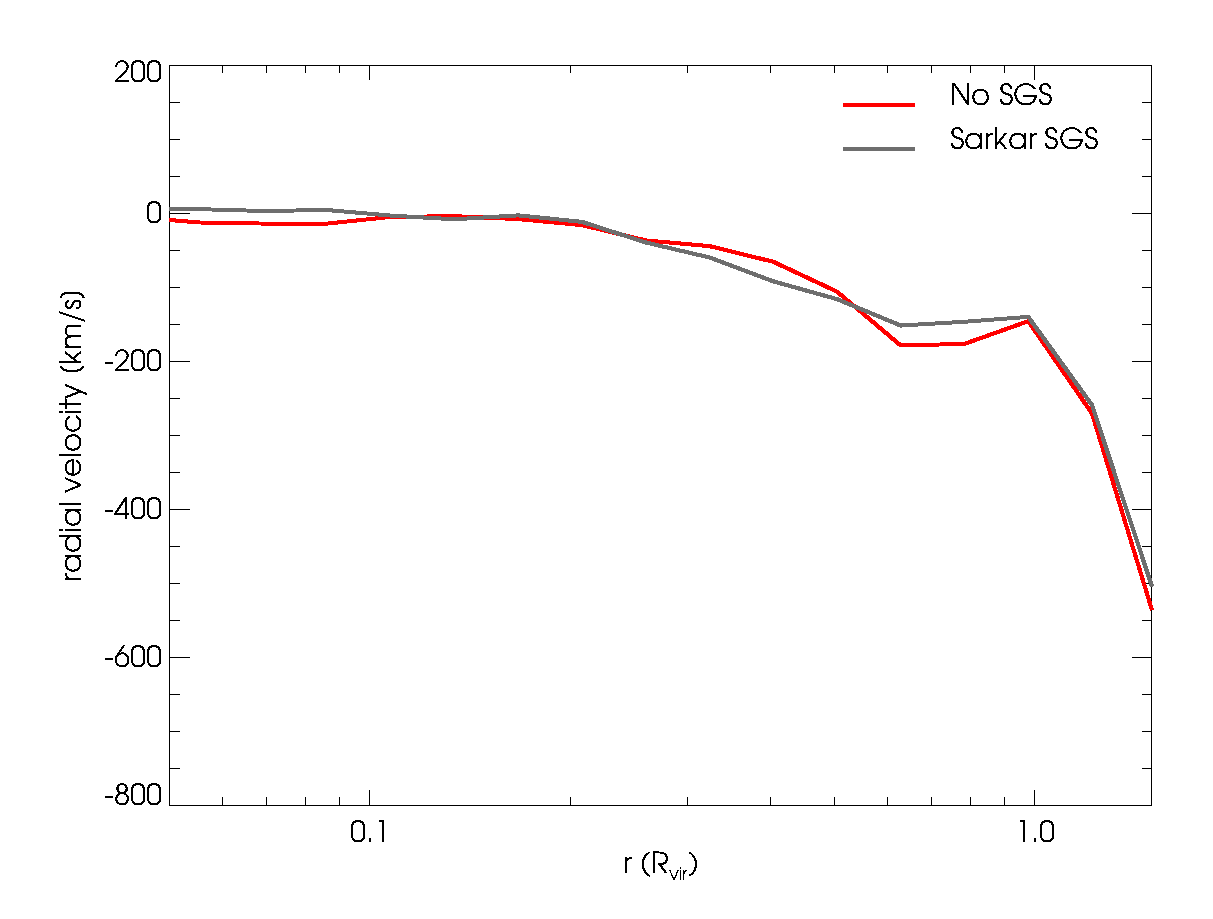
\includegraphics[width=0.45\linewidth]{chapter9/vradlog.eps}
\label{fig:vrad}}
\subfigure[Radial averaged velocity dispersion.]{
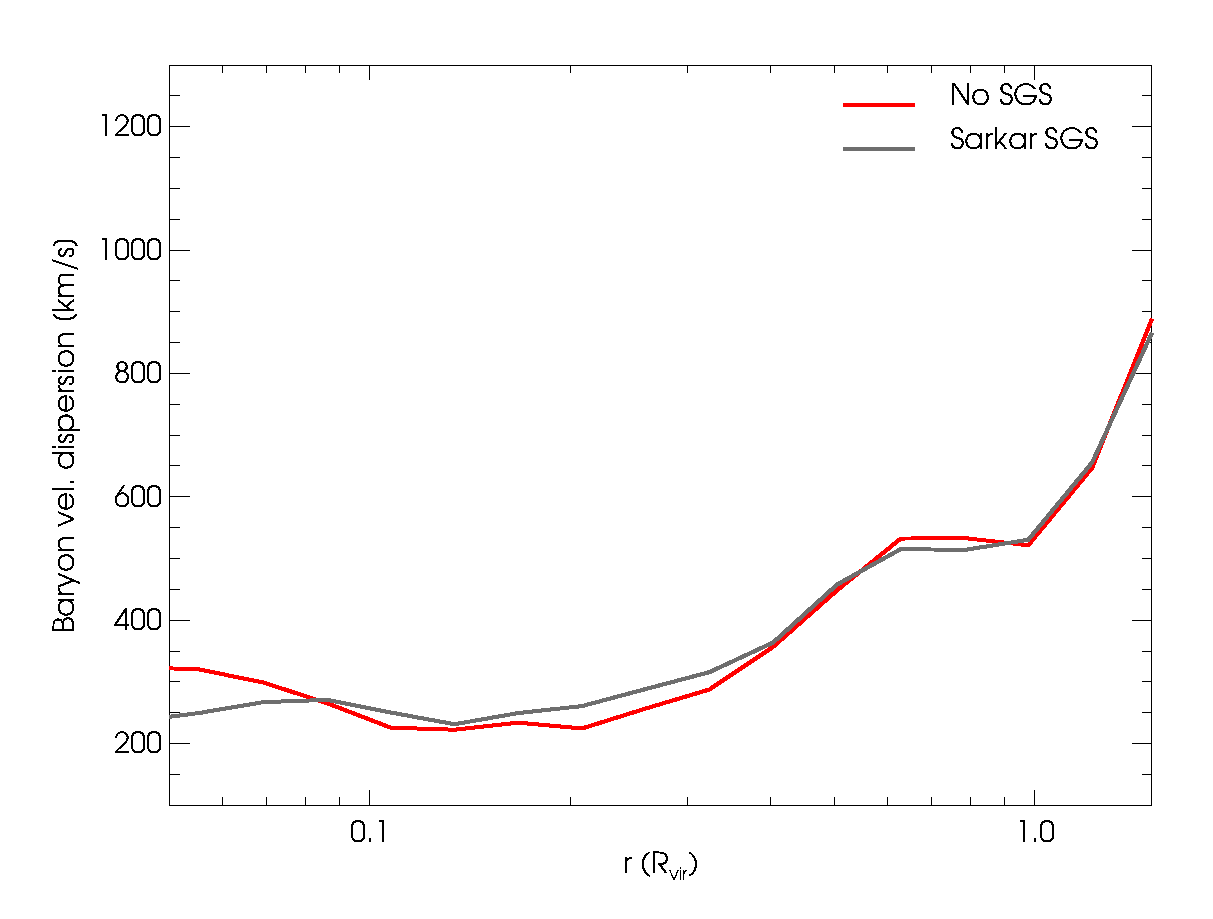
\includegraphics[width=0.45\linewidth]{chapter9/sigma_gaslog.eps}
\label{fig:sigma}}
\subfigure[Scaled turbulent velocity.]{
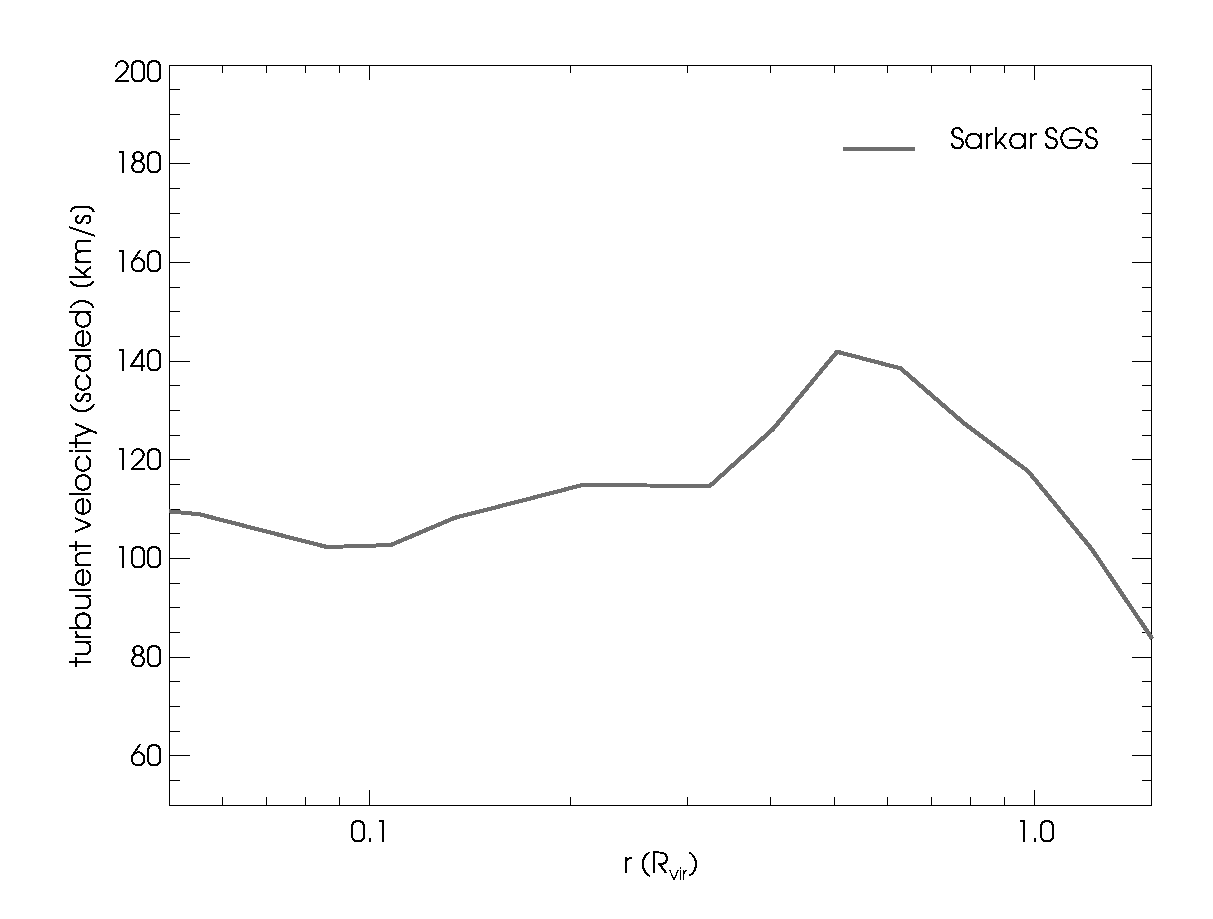
\includegraphics[width=0.7\linewidth]{chapter9/vturblog.eps}
\label{fig:vturb}}
\caption{Radial profiles of several velocity related quantities around the
center of the galaxy cluster. The results for the simulation with and without
Sarkar SGS model are plotted in red and black respectively.}
\end{figure}

The plots show the mass weighted average values at radius $r$ of temperature
$T(r)$ in Kelvin, the density\footnote{The density is not mass weighted
.} $\rho(r)$ in $\unit{M_{\odot}/Mpc^3}$, the scaled turbulent velocity
according to equation \eqref{eq:vturbscaled} $v_t(r)$ in $\unit{km\ s^{-1}}$,
the radial component of the resolved velocity $v_r(r)$ in $\unit{km\ s^{-1}}$,
the entropy $K$ in code units, which is defined as\footnote{This definition of
entropy is often used in literature on galaxy clusters
\citep{Voit2005,Iapichino2008}.}
\begin{align}
K=\frac{T}{\rho^{\gamma-1}}
\end{align}
with $\gamma = 5/3$, the x-ray luminosity $L_X \sim \rho^2 T^{1/2}$ and the
radially averaged velocity dispersion, which is defined as the standard
deviation of the velocity averaged over a spherical shell as
\begin{align}
\sigma(r) = \frac{\sum_i m_i \lra{v_i - \fil{v(r)}}^2}{\sum_i m_i} 
\end{align}
where $\fil{v(r)} = \frac{\sum_i m_i}{\sum_i m_i}$ is the mass weighted mean
value of velocity in the spherical shell at radius $r \pm \delta r$. 

At first it is apparent from these plots that, except for the radial
component of the resolved velocity, the run with SGS model only shows
significant deviations from the run without SGS model in the cluster core at
$r<0.1\ R_{vir}$. However since \texttt{enzo\_anyl} proved not to be
robust for 
$r< 0.07\ R_{vir}$ \citep{Iapichino2008}, one cannot use the values
obtained by these plots for a consistent analysis of the cluster core; this
will be done in the next chapter using a different tool.
Nevertheless the general trend from these plots is, that the SGS model lowers
the entropy in the core, which leads to a higher density and a lower
temperature in the center of the cluster. Since the X-ray luminosity is
proportional to $\rho^2$, it is higher in the cluster core of the simulation
with SGS model. Looking more precisely at the radial profile of entropy
(fig. \ref{fig:entro}), one can also see that in the simulation without the SGS
model, the entropy inside the core of the cluster $r > 0.1\ R_{vir}$ is
basically constant, which suggests that the gas is adiabatic there. With the
SGS model this is not the case; the entropy is falling steadily towards the
center of the core. 

The last observation can be discussed more quantitatively in terms of
polytropic processes. A polytropic process is defined as a process, where
\begin{align}
\frac{T}{\rho^{n-1}} = const.,
\end{align}
where $n$ is called the polytropic index. By reversing that logic we can
compute an effective polytropic $n_{\text{eff}}(r)$ index by demanding that
\begin{align}
\td{r}\lra{\frac{T}{\rho^{n_{\text{eff}}(r)-1}}}=0,
\end{align}
which leads to
\begin{align}
n_{\text{eff}}(r)=\frac{\rho}{T}\frac{\ttd{r}{T}}{\ttd{r}{\rho}}+1
=\ttd{\ln T}{\ln \rho}+1. 
\end{align}
In figure \ref{fig:poly}
we show a plot of the radial dependence of the effective
polytropic index for our two simulations with and without SGS model. 
We see that the polytropic index in the simulation without SGS
model is $n_{\text{eff}} \approx 1.7$, which is near to the adiabatic case
$n_{\text{eff}} \approx 5/3$, as expected. The simulation with SGS model is
clearly not
adiabatic, with $n_{\text{eff}} \approx 1.3 \approx 4/3$ in the center. We
also note that at a radius $r \approx 0.2\ R_{vir}$, the gas behaves
basically
isothermal, which can also be seen in the temperature profile
(figure \ref{fig:temp}). At an even bigger distance from the core 
$r > 0.2\ R_{vir}$, the cluster gas in both simulations behaves similarly,
with a
polytropic index rising from $n \approx 1.3$ to $n \approx 1.4$. 
If we compute an average polytropic index over the region 
$0.05\ R_{vir} < r < 1.0\ R_{vir}$ we get $n_{\text{eff}} = 1.27$
and $n_{\text{eff}} = 1.18$
for the simulation without and with SGS respectively. It is
interesting to compare these values with results from observations. For example 
\citet{Markevitch1998} found that they could fit their measured temperature
profiles with a polytropic index of $n=1.2-1.3$, which would fit reasonably
well to our average values. However, \citet{Pratt2002} claim that 
$n=1.07 \pm 0.1$ is the best fit to their observed temperature profile, and
therefore state, that the whole cluster can be seen as nearly isothermal.
But newer measurements by \citet{Vikhlinin2006} now reveal, that the
temperature profile cannot be fitted by a single polytropic index in agreement
with our analysis. \citet{Vikhlinin2006} also find a broad plateau of
temperature at $r=0.2\ R_{vir}$ in most of their clusters, however all
their
temperature profiles show a decline of temperature towards the center of the
cluster at $r < 0.2\ R_{vir}$, a so-called "cool core". This feature
could
neither be reproduced by the simulation without SGS nor with SGS. It seems like
including turbulence alone in a cluster simulation cannot be a solution to the
"cool core" problem. 

The radial resolved velocity is not changed significantely by
the SGS model, but comparing this plot with the radial profile of the turbulent
velocity the following picture emerges: From a radius $r > R_{vir}$
material is falling onto the cluster, being decelerated strongly at the
virial radius $r = R_{vir}$ (see drop of radial velocity at this point in
figure \ref{fig:vrad}). This deceleration leads to a steady rise in turbulent
energy at $r<R_{vir}$ up to a peak at $r=0.5\ R_{vir}$ followed by a drop of to
a quite stable value of $\sim \unit[110]{km s^{-1}}$ in the region 
$r<0.3\ R_{vir}$. One might want to compare these value to the velocity
dispersion, however these values are not comparable directly. The turbulent
velocity depicted in the plot is computed for the characteristic scale
$\unit[15.7]{kpc\ h^{-1}}$, which is constant with the radius. The velocity
dispersion is the deviation of velocity in a spherical shell at radius $r$, so
the characteristic scale of $\sigma$ is basically the circumference of this
shell
$l=2\pi r$, which is of course not independent of the radius. Therefore we
cannot interpret the value of $\sigma$ in the same local sense as we can do for
the other quantities. We therefore doubt that it is useful to draw conclusions
about the local nature of turbulence from a plot like fig. \ref{fig:sigma}, as
is often done in the literature (e.g. \citep{Norman1999a}). 

\subsection{Spatial distribution of turbulent energy}
To investigate the time development of the spatial distribution of turbulent
energy, we generated slices of density and turbulent energy with the graphical
analysis tool VisIt. 
\begin{figure}[tp]
\centering
\subfigure[$z=0.15$.]{
\includegraphics[width=0.46\linewidth,clip,trim=150 50 50 0]
{chapter9/mergerdens0011.eps}
\label{fig:dens0011}}
\subfigure[$z=0.15$.]{
\includegraphics[width=0.46\linewidth,clip,trim=150 50 50 0]
{chapter9/mergereturb0011.eps}
\label{fig:eturb0011}}
\subfigure[$z=0.1$.]{
\includegraphics[width=0.46\linewidth,clip,trim=150 50 50 0]
{chapter9/mergerdens0012.eps}
\label{fig:dens0012}}
\subfigure[$z=0.1$.]{
\includegraphics[width=0.46\linewidth,clip,trim=150 50 50 0]
{chapter9/mergereturb0012.eps}
\label{fig:eturb0012}}
\caption{Slices of density (left) and turbulent energy at a length scale of
$\unit[15.6] {Mpc\ h^{-1}}$ (right) at varying redshifts $z$. The color coding
shows both quantities in code units using a logarithmic scaling. The overlayed
contours show density and the overlayed vector field depicts the strength and
direction of the baryonic velocity field in code units using a linear scale. The
slices show a 
region of $\unit[6.4 \times 6.4] {Mpc\ h^{-1}}$. }
\end{figure}
\begin{figure}[tp]
\centering
\subfigure[$z=0.05$.]{
\includegraphics[width=0.46\linewidth,clip,trim=150 50 50 0]
{chapter9/mergerdens0013.eps}
\label{fig:dens0013}}
\subfigure[$z=0.05$.]{
\includegraphics[width=0.46\linewidth,clip,trim=150 50 50 0]
{chapter9/mergereturb0013.eps}
\label{fig:eturb0013}}
\subfigure[$z=0$.]{
\includegraphics[width=0.46\linewidth,clip,trim=150 50 50 0]
{chapter9/mergerdens0014.eps}
\label{fig:dens0014}}
\subfigure[$z=0$.]{
\includegraphics[width=0.46\linewidth,clip,trim=150 50 50 0]
{chapter9/mergereturb0014.eps}
\label{fig:eturb0014}}
\caption{Slices of density (left) and turbulent energy at a length scale of
$\unit[15.6] {Mpc\ h^{-1}}$ (right) at varying redshifts $z$. The color coding
shows both quantities in code units using a logarithmic scaling. The overlayed
contours show density and the overlayed vector field depicts the strength and
direction of the baryonic velocity field in code units using a linear scale. The
slices show a region of $\unit[6.4 \times 6.4] {Mpc\ h^{-1}}$. }
\end{figure}
The slices are taken around the place of
formation of our main galaxy cluster and show a region of size 
$\unit[6.4 \times 6.4] {Mpc\ h^{-1}}$. Overlayed onto the slices are density
contour lines and a vector field showing the strength and direction of
the velocity. In the density slice at redshift $z=0.15$
(figure \ref{fig:dens0011}), we can see from the velocity vectors that material
is falling onto the cluster along filament from the lower left and from the
upper right corner. But from the upper right corner we do not have a smooth
inflow of matter, instead two small clumps are approaching. Over the course of
the simulation these two clumps merge with the main cluster
(figure \ref{fig:dens0012}-\ref{fig:dens0012}) and are assimilated completely
at redshift $z=0$. Only the velocity field still shows some disturbance
due to the infalling clumps.  

In the slice of the turbulent energy (figure \ref{fig:eturb0011}) at $z=0.15$,
we see a hot spot of turbulent energy in the center of our cluster, which is due
to a former major merger. The turbulent energy produced due to this merger is
declining (figure \ref{fig:eturb0012}-\ref{fig:eturb0014}) and at redshift
$z=0$ it is presumably dissipated into internal energy completely, so there
is only little turbulent energy left at the center of the cluster. 

However the two approaching clumps will drive turbulence again in the cluster.
Thereby the left clump can be identified in the turbulent energy slice at
$z=0.15$ (figure \ref{fig:eturb0011}) as a ring-like structure, showing that
turbulence is not produced in the center of the infalling clump, but is
presumably produced at the front (behind a 
bow shock) and in the wake of the infalling material. But the right clump only
shows some turbulence production in its wake, which might be due to its smaller
size and smaller velocity. However, on their way towards the main cluster, both
clumps develop a hot spot of turbulent energy (figure
\ref{fig:eturb0012}-\ref{fig:eturb0013}). The hot spot of turbulent energy can
even be identified after the two clumps have merged with the main cluster
(figure \ref{fig:eturb0014}) and are not visible in the density slice (figure
\ref{fig:dens0014}) anymore. In this sense,
the distribution of turbulent energy traces the local merging history of a
galaxy cluster until it is dissipated into heat completely. Also the merging of
the two small clumps with the main cluster drives turbulence only in its
outer rim, showing that smaller mergers might only be able to drive turbulence
in the outer regions ($r > R_{vir}$) of a cluster. But turbulence is
sustained for a longer time in a galaxy cluster than one might expect from just
looking at density development.

\subsection{Cluster core analysis}
As mentioned we couldn't use the \texttt{enzo\_anyl} tool to compute average
values of
thermodynamic quantities of the cluster core. Instead we analyzed the cluster
core using the interactive parallel visualization and graphical analysis tool
VisIt\footnote{Freely available from https://wci.llnl.gov/codes/visit.}. Using
this tool we computed several mass-weighted averaged quantities within a sphere
of radius $R=0.1\ R_{vir}$, centered at the cluster center. The results of this
analysis are summarized in tables
\ref{tab:avg}\subref{tab:avg1}-\ref{tab:avg}\subref{tab:avg3}.
\begin{table}[tp]
\begin{center}
\begin{small}
\subtable[General quantities.]{
\begin{tabular}{lccccc}
\hline
Run & $m_{bar}$ & $\rho$ & $T$ & $K$ & $\sigma$\\
& $[\unit[]{10^{12}\ M_{\odot}}]$
& $[\unit[]{10^{14}\ M_{\odot}\ Mpc^{-3}}]$
& $[\unit[]{10^7\ K}]$
& $[\unit[]{10^5 \times code\ units}]$
& $[\unit[]{km\ s^{-1}}]$\\
\hline
no SGS & 2.73 & 0.996 & 7.88 & 4.40 & 200\\
SGS & 3.37 & 1.29 & 6.99 & 3.38 & 257\\
\hline
\end{tabular}
\label{tab:avg1}
}
\\
\subtable[Resolved and thermal pressure.]{
\begin{tabular}{lccccc}
\hline
Run 
& $p_{th}/\rho$ 
& $p_{res}/\rho$ 
& $\frac{p_{res}}{p_{th}+p_{res}}$\\
& $[\unit[]{10^{16}\ cm^2 s^{-2}}]$
& $[\unit[]{10^{14}\ cm^2 s^{-2}}]$
& $[\unit[]{\%}]$\\
\hline
no SGS & 1.05 & 1.34 & 1.25\\
SGS & 0.936 & 2.20 & 2.30\\
\hline
\end{tabular}
\label{tab:avg2}
}
\\
\subtable[SGS quantities.]{
\begin{tabular}{lccccc}
\hline
Run 
& $p_{turb}/\rho$ 
& $\epsilon$ 
& $\Sigma$\\
& $[\unit[]{10^{14}\ cm^2 s^{-2}}]$
& $[\unit[]{10^{-5}\ cm^2 s^{-3}}]$
& $[\unit[]{10^{-5}\ cm^2 s^{-3}}]$\\
\hline
no SGS & 0.0 & 0.0 & 0.0\\
SGS & 0.380 & 3.06 & 2.92\\
\hline
\end{tabular}
\label{tab:avg3}
}
\end{small}
\end{center}
\caption{Mass weighted values of some quantities, calculated
within a sphere with $R = 0.1\ R_{vir}$ centred at the cluster center at
z=0.}
\label{tab:avg}
\end{table}
The table lists as general quantities of the simulations the baryonic mass
$m_{bar}$ inside the chosen sphere, the density $\rho$, the temperature $T$, the
entropy $K=\frac{T}{\rho^{\gamma-1}}$ with $\gamma=5/3$ and the baryonic
velocity dispersion $\sigma= \frac{\sum_i m_i \lra{v_i -
\fil{v}}^2}{m_{bar}}$ at the length scale 
$l=0.1\ R_{vir}=\unit[133]{kpc\ h^{-1}}$. According to \citet{Voit2005} entropy
is the most important quantity to look at, because it determines
the structure of the intracluster medium and it records the thermodynamic
history of the cluster's gas; the temperature and density are just
manifestations of the entropy.
We find that the ratio of the entropies in the cluster core of the two
simulations (in the 
following 1 is used to subscript quantities of the run without SGS model, 2
subscripts quantities of the simulation with SGS model) is
\begin{align}
\frac{K_1}{K_2}=1.30 = \lra{\frac{\rho_1}{\rho_2}}^{-1}=
\lra{\frac{\sigma_1}{\sigma_2}}^{-1}.
\end{align}
Since $\frac{K_1}{K_2}=
\lra{\frac{T_1}{T_2}}\lra{\frac{\rho_1}{\rho_2}}^{-2/3}$ by definition, this
yields
\begin{align}
\lra{\frac{T_1}{T_2}}=\lra{\frac{\rho_1}{\rho_2}}^{-1/3}=1.09,
\end{align}
which is roughly fulfilled, since from the data directly
we get $T_1/T_2 = 1.13$. So temperature and density are really just
manifestations of entropy, but also the velocity dispersion of the baryonic
gas in the cluster core seems to be directly connected to the entropy.
Because of this, the velocity dispersion at a length scale of $l=0.1\ R_{vir}$
in
the simulation with the SGS model is significantely higher than in the
simulation without SGS model.

In table \ref{tab:avg2} we list the thermodynamic pressure $p_{th}$ and the
resolved pressure, which is defined as
\begin{align}
p_{res}=\frac{1}{3} \rho \sigma^2,
\end{align}
and the ratio between resolved and thermodynamic pressure. We see that, in 
the case of the SGS model simulation, the ratio of resolved to thermal pressure
is nearly twice as high compared to the simulation without SGS model, since
density and velocity dispersion are higher in the core when using the SGS
model.

Listed in table \ref{tab:avg3} is also the turbulent pressure, defined as
\begin{align}
p_{res}=\frac{1}{3} \rho q^2,
\end{align}
where $q^2$ is related to the velocity fluctuations at grid length scale 
$l=\unit[15.7]{kpc\ h^{-1}}$. So directly comparing or adding the resolved
pressure to the turbulent pressure is not useful, since both are related to the
deviations of the velocity on different length scales. However,
the ratio of turbulent production $\Sigma$ to turbulent dissipation $\epsilon$
in the core of the cluster is interesting
\begin{align}
\frac{\Sigma}{\epsilon}=0.95,
\end{align}
showing that we are actually in a regime of near equilibrium of production and
dissipation of turbulent energy, a sign that a turbulent cascade has
established.

\subsection{Influence of SGS parameters on cluster core}
In an attempt to better understand the influence of the SGS model on the
thermodynamic properties of the cluster core, we conducted a series of
simulations with different parameters for the SGS model. Because of our
restricted CPU budget we could not afford to do these simulations with the full
$128^3$ root grid resolution, rather we were only able to do these studies using
a
root grid resolution of $32^3$ grid cells and $32^3$ N-body particles. In
analogy to the high resolution simulation, we also nested a static child grid
inside the root grid, with $32^3$ cells and $32^3$ N-body particles. The mass
of each particle in this grid was $\unit[5.8 \times 10^{11}]{M_{\odot}\
h^{-1}}$,
so the resolution of the gravitational potential due to dark matter was much
lower in these runs. We allowed adaptive grid refinement from level
$l=2$ to $l=8$ in a volume of $\unit[38.4]{Mpc\ h^{-1}}$ inside this grid, so
the effective resolution of the baryonic component and all the other
parameters were equal to the high resolution runs.
The galaxy clusters that formed in these simulations had a virial mass of
roughly $M_{vir}=\unit[6.9 \times 10^{14}]{M_{\odot}\ h^{-1}}$ and a virial
radius
of $R_{vir}=\unit[1.27]{Mpc\ h^{-1}}$.

\begin{figure}[tp]
\centering
\subfigure[Linear scaling.]{
\includegraphics[width=0.45\linewidth]{chapter9/epsfitturb.eps}
\label{fig:epsfit}}
\subfigure[Logarithmic scaling.]{
\includegraphics[width=0.45\linewidth]{chapter9/epsfitturblog.eps}
\label{fig:epsfitlog}}
\caption{Plot of turbulent pressure over density versus turbulent dissipation
in the center of the cluster core for different parameters of the SGS model.}
\end{figure}

As parameters we chose all combination of $C_{\nu} = (0.0, 0.05),
C_{\lambda}=(0.0,-0.2),C_{\mathbb{D}}=(0.0,0.4)$ and $C_p =
(0.0,1.0)$\footnote{Setting $C_p=0.0$ means switching off
the influence of the turbulent pressure in the momentum equation.}, which 
gave use 16 combinations altogether. In complete analogy to the high resolution
runs we analyzed the average values of thermodynamic quantities of the cluster
core. Albeit one interesting preliminary result emerged. By plotting the 
average values of the turbulent pressure over the average value of turbulent
dissipation in the cluster core (figures \ref{fig:epsfit},\ref{fig:epsfitlog}),
we found that they seem to be related as
\begin{align}
\fil{\frac{p_t(l_{min})}{\rho}} = 
C (\fil{\epsilon} R_{vir})^{2/3},\label{eq:turbeos}
\end{align}
where $\fil{}$ means the mass weighted average over the cluster core
$r<0.1\ R_{vir} $, $l_{min}=\unit[15.6]{kpc\ h^{-1}}$ and $R_{vir} =
\unit[1.27]{Mpc\ h^{-1}}$. The constant $C$ can be found
from a linear fit to be $C \approx 1$ (see fit in figures
\ref{fig:epsfit},\ref{fig:epsfitlog}).
If we use again our scaling relation for the
turbulent velocity \eqref{eq:vturbscaled}, we get with
$\fil{\frac{p_t(l_{min})}{\rho}} = \fil{q^2(l_{min})}$ and $C=1$
\begin{align}
\fil{q^2(l)} = \lra{\frac{R_{vir}}{l_{min}}}^{2/3} \fil{\epsilon}^{2/3} l^{2/3}
\end{align}
If we assume, that the value of $\frac{R_{vir}}{l_{min}}^{2/3} = 18.8$ is
universal, we get for cluster core turbulence the relation
\begin{align}
\fil{q^2(l)} = 18.8 \fil{\epsilon}^{2/3} l^{2/3}.
\end{align}
In this sense, we can interpret $C_{k,core}=18.8$ as a Kolmogorov constant for
the cluster core turbulence, which is more than 10 times higher than what is
found for the Kolmogorov constant in simulations of incompressible turbulence.


